\chapter{Introducción a las Trenzas}
\label{ch::capitulo1}

\section{Concepto intuitivo de Trenza}

Imaginemos varias cuerdas colgando verticalmente, cada una fijada en sus extremos superior e inferior. Una \textbf{trenza} se crea cuando estas cuerdas se cruzan entre sí siguiendo un patrón específico de entrelazado. A diferencia de los nudos, en una trenza no cerramos las cuerdas en un ciclo; simplemente las reordenamos mediante una serie de cruces.

\begin{figure}[h!]
    \centering
    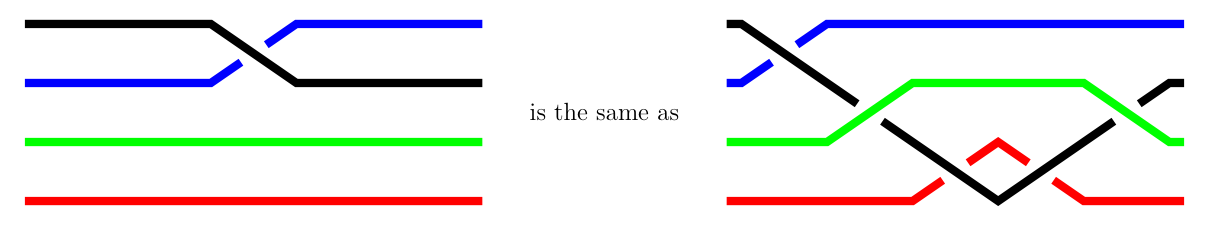
\includegraphics[width=0.6\textwidth]{figures/chapters/1_def_grupo/trenzas_equivalentes.png}
    \caption{Trenzas equivalentes Fuente: \cite{ArithmeticBraids}}
\end{figure}

Un \textbf{diagrama de trenzas} es una representación visual en la que los cruces entre las cuerdas se muestran como puntos de intersección. En cada cruce, una cuerda pasa sobre o bajo otra. Estos diagramas permiten visualizar y manipular trenzas de manera matemática.

% Por ejemplo, si tenemos tres cuerdas, etiquetadas como \(1\), \(2\), y \(3\), una trenza puede formarse cruzando la cuerda \(1\) sobre la cuerda \(2\) y luego cruzando la cuerda \(2\) sobre la cuerda \(3\). La secuencia y el orden de estos cruces son fundamentales para definir la estructura de la trenza.

% \section{Notación de Artin y Generadores \(\sigma_i\)}

% Para describir una trenza de forma algebraica, usamos la \textbf{notación de Artin}, que introduce \textbf{generadores} \(\sigma_i\) que representan cruces específicos:

% \begin{itemize}
%     \item \(\sigma_i\): Este símbolo indica un cruce en el cual el hilo \(i\) pasa \textbf{por encima} del hilo \(i+1\).
% \end{itemize}

% \textbf{Ejemplo:} En una trenza con tres hilos, tenemos dos generadores: \(\sigma_1\) y \(\sigma_2\).
% \begin{itemize}
%     \item \(\sigma_1\) representa un cruce donde el hilo \(1\) pasa sobre el hilo \(2\).
%     \item \(\sigma_2\) representa un cruce donde el hilo \(2\) pasa sobre el hilo \(3\).
% \end{itemize}

% Una trenza puede representarse mediante una secuencia de generadores. Por ejemplo, la secuencia \(\sigma_1 \sigma_2 \sigma_1\) representa una trenza en la que:
% \begin{enumerate}
%     \item Primero, el hilo \(1\) cruza sobre el hilo \(2\).
%     \item Luego, el hilo \(2\) cruza sobre el hilo \(3\).
%     \item Finalmente, el hilo \(1\) vuelve a cruzar sobre el hilo \(2\).
% \end{enumerate}

% Esta notación simplifica el estudio de las trenzas, permitiendo describir la estructura de una trenza de forma algebraica.

\section{Definición del Grupo de Trenzas \( B_n \)}

El \textbf{grupo de trenzas} \( B_n \) es el conjunto de todas las configuraciones posibles de trenzas con \( n \) hilos. Cada elemento de \( B_n \) representa una disposición particular de los hilos, determinada por una secuencia de cruces.

En \( B_n \), podemos combinar (o «concatenar») dos trenzas para obtener otra trenza en \( B_n \), donde la secuencia de cruces de una trenza sigue a la otra. Esta operación de concatenación, junto con ciertas propiedades que detallaremos en la siguiente sección, le da a \( B_n \) una estructura de grupo algebraico.

Estudiaremos con más detalle las relaciones algebraicas de \( B_n \), incluyendo las relaciones de Artin, en el próximo capítulo. Por ahora, nos enfocaremos en por qué \( B_n \) cumple con las propiedades de un grupo.

\subsection{Las Trenzas como generalización del Grupo Simétrico \( S_n \)}

Para comprender el grupo de trenzas \( B_n \), primero necesitamos conocer el \textbf{grupo simétrico} \( S_n \), que es el grupo de todas las permutaciones de \( n \) elementos. Una permutación es una reorganización de elementos en un cierto orden, y el grupo \( S_n \) representa todas las posibles formas de reorganizar \( n \) elementos mediante permutaciones.

El grupo \( S_n \) describe cómo se pueden reorganizar los elementos, pero no incluye información sobre \textbf{cómo se realiza el proceso de reorganización}. En otras palabras, \( S_n \) muestra el resultado final de la permutación, pero no el camino o el orden de las operaciones específicas para llegar a esa permutación.

\begin{figure}[h!]
    \centering
    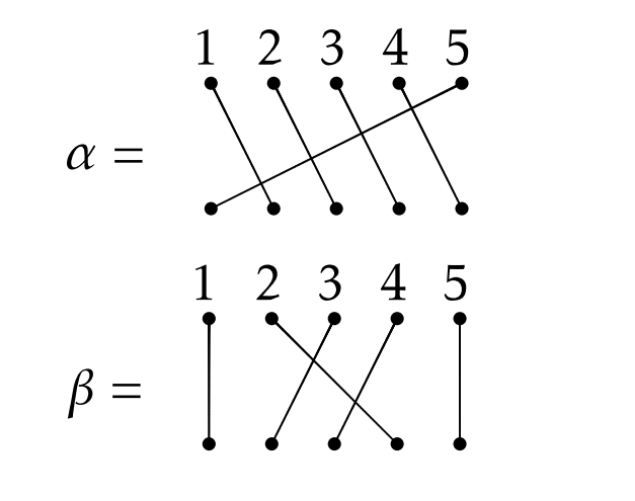
\includegraphics[width=0.4\textwidth]{figures/chapters/1_def_grupo/symmetric_group.png}
    \caption{Ejemplo de elementos del grupo simétrico $S_5$. Fuente: \cite{ernst_43_2022}}
    \label{fig:ciclo_5}
\end{figure}

\bigskip

El grupo de trenzas \( B_n \) puede considerarse una \textbf{generalización} de \( S_n \) porque no solo especifica el resultado final de reorganizar los \( n \) hilos, sino también el orden de los cruces. En \( B_n \), podemos especificar si un hilo pasa \textbf{por encima} o \textbf{por debajo} de otro al cruzarse, lo cual agrega un nivel adicional de detalle.

\begin{figure}[h!]
    \centering
    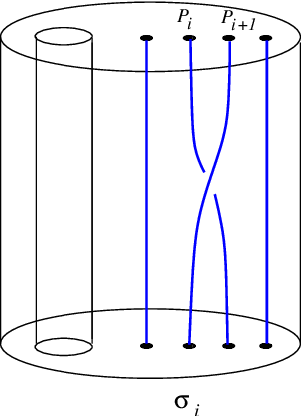
\includegraphics[width=0.25\textwidth]{figures/chapters/1_def_grupo/op_braid.png}
    \caption{Ejemplo de una trenza. Fuente: \cite{vershinin_about_2014}}
    \label{fig:operacion_simple_trenza}
\end{figure}

% Por ejemplo, en \( B_4 \) (el grupo de trenzas de cuatro hilos), la imagen \ref{fig:operacion_simple_trenza} muestra una trenza en la que el hilo \( P_i \) cruza sobre el hilo \( P_{i+1} \). Este tipo de cruce representa los generadores de \( B_4 \), donde \( \sigma_i \) indica que el hilo \( i \) cruza sobre el hilo \( i+1 \).

En \( B_n \), la \textbf{dirección y el orden} de los cruces son importantes, lo que distingue a \( B_n \) de \( S_n \), ya que \( B_n \) permite configuraciones más detalladas que las simples permutaciones de \( S_n \).

\bigskip

En resumen, \( S_n \) se enfoca en el resultado final de una reorganización, mientras que \( B_n \) toma en cuenta el proceso completo, incluyendo el orden de los cruces y si los hilos pasan por encima o por debajo. Esto hace que el grupo de trenzas \( B_n \) sea una extensión o generalización del grupo simétrico \( S_n \).

\subsection{Propiedades de grupo}

\subsubsection{Clausura}

La propiedad de \textbf{clausura} significa que, al combinar dos elementos cualesquiera del grupo, el resultado es otro elemento dentro del mismo grupo. En el caso de \( B_n \), esto implica que si tomamos dos trenzas cualesquiera en \( B_n \) y las concatenamos, el resultado es otra trenza en \( B_n \).

Visualmente, si tenemos dos trenzas, \( B_1 \) y \( B_2 \), la concatenación de \( B_1 \) seguida de \( B_2 \) produce una trenza que también pertenece al grupo \( B_n \).

\subsubsection{Asociatividad}

La operación de concatenación en \( B_n \) es \textbf{asociativa}. Esto significa que, para cualquier trenzas \( B_1 \), \( B_2 \), y \( B_3 \), se cumple que:
\[
(B_1 \cdot B_2) \cdot B_3 = B_1 \cdot (B_2 \cdot B_3).
\]

\begin{figure}[h!]
    \centering
    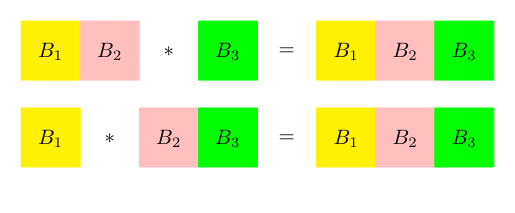
\includegraphics[width=0.7\textwidth]{figures/chapters/1_def_grupo/asociativa.png}
    \caption{Propiedad asociativa en el grupo de trenzas. Fuente: \cite{ArithmeticBraids}}
    \label{fig:propiedad_asociativa}
\end{figure}

Esta propiedad se ilustra en la imagen \ref{fig:propiedad_asociativa}, donde los rectángulos de colores representan trenzas arbitrarias \( B_1 \), \( B_2 \), y \( B_3 \). La figura muestra que, independientemente de cómo se agrupen las trenzas al concatenarlas, el resultado final es el mismo. Esta es una propiedad clave de los grupos y es fundamental para la estructura de \( B_n \).

\subsubsection{Elemento identidad}

En \( B_n \), existe una trenza especial llamada \textbf{elemento identidad}, que denotamos como \( I \). La trenza identidad está formada por \( n \) hilos paralelos sin cruces. Al concatenar cualquier trenza \( B \) con \( I \), el resultado es la misma trenza \( B \):
\[
B \cdot I = I \cdot B = B.
\]

\begin{figure}[h!]
    \centering
    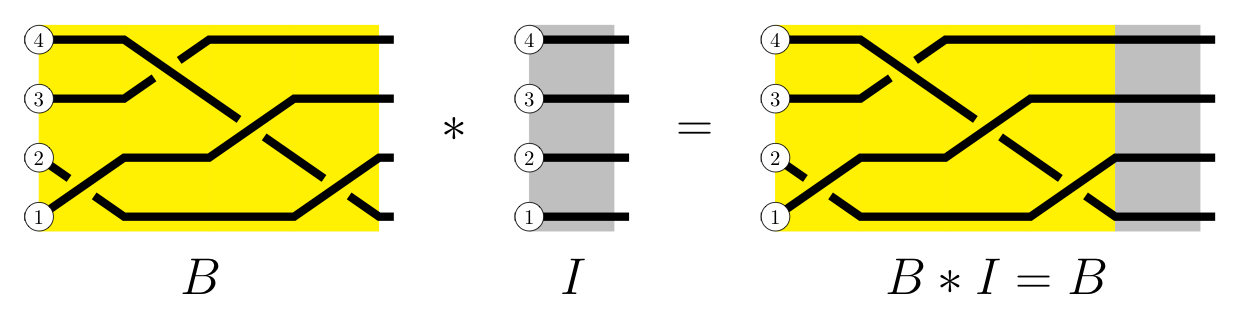
\includegraphics[width=0.7\textwidth]{figures/chapters/1_def_grupo/elemento_neutro.png}
    \caption{Elemento identidad en el Grupo de Trenzas $B_4$. Fuente: \cite{ArithmeticBraids}}
    \label{fig:elemento_neutro}
\end{figure}

En la imagen \ref{fig:elemento_neutro}, el elemento identidad se representa como una trenza sin cruces. Cuando concatenamos esta trenza con otra trenza \( B \), el resultado es idéntico a \( B \), lo cual cumple la propiedad de identidad.

\subsubsection{Elemento inverso}

Cada trenza en \( B_n \) tiene un \textbf{elemento inverso} que deshace sus cruces. Esto significa que, para cualquier trenza \( B \), existe otra trenza \( B^{-1} \) tal que:
\[
B \cdot B^{-1} = B^{-1} \cdot B = I,
\]
donde \( I \) es la trenza identidad.

\begin{figure}[h!]
    \centering
    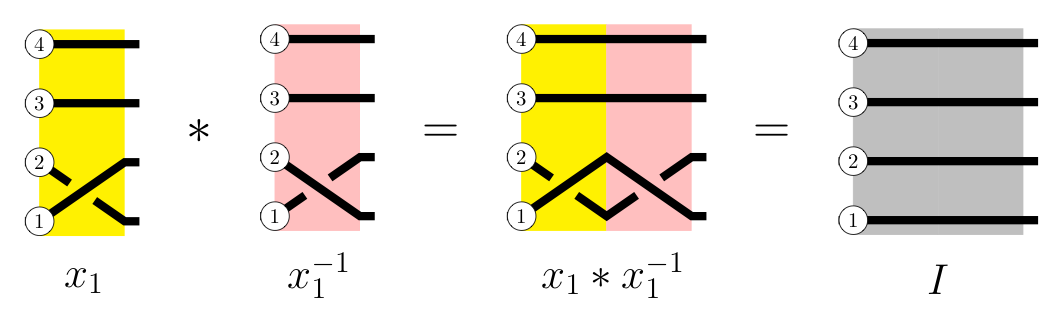
\includegraphics[width=0.7\textwidth]{figures/chapters/1_def_grupo/elemento_inverso1.png}
    \caption{Elemento inverso en el Grupo de Trenzas $B_4$. Fuente: \cite{ArithmeticBraids}}
    \label{fig:elemento_inverso}
\end{figure}

En las imágenes proporcionadas, se muestra cómo una trenza \( B \) y su inverso \( B^{-1} \) se combinan para dar como resultado la trenza identidad. Este concepto puede visualizarse imaginando una serie de cruces que se deshacen en orden inverso, dejando los hilos en su posición original, sin entrelazarse.

% TODO Incluir en la parte de Artin
% \begin{figure}[h!]
%     \centering
%     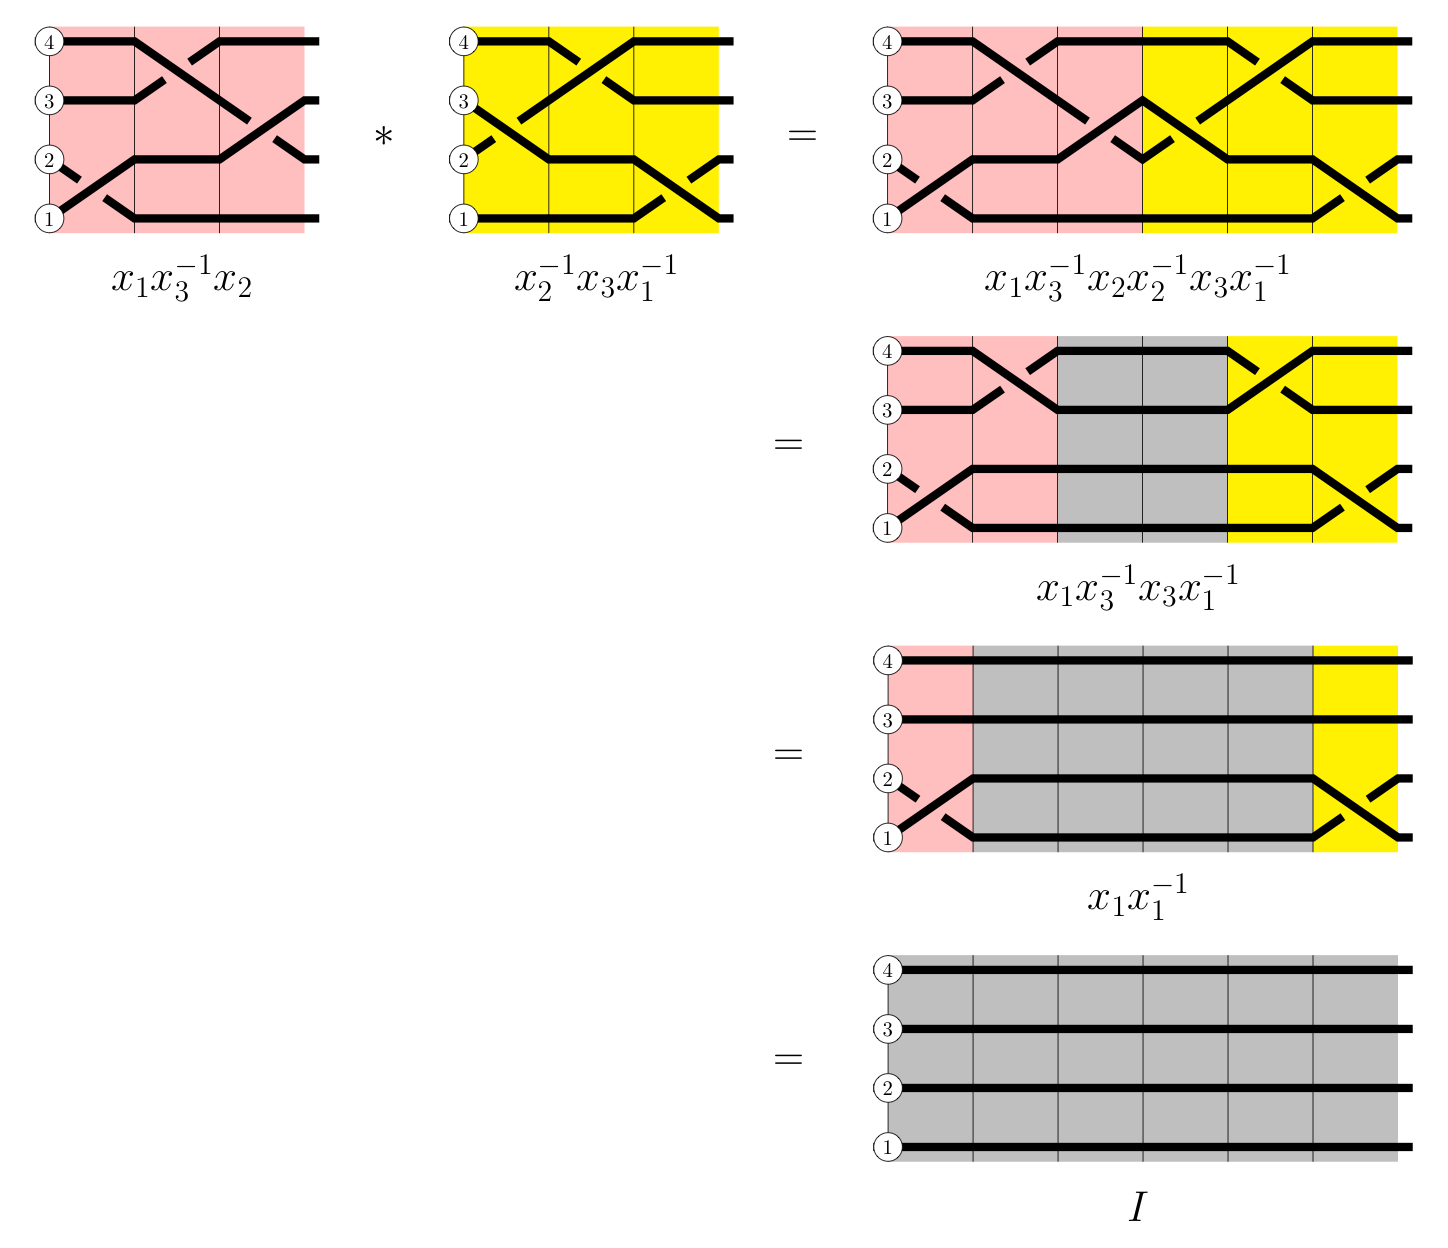
\includegraphics[width=0.6\textwidth]{figures/chapters/1_def_grupo/elemento_inverso2.png}
%     \caption{Proceso de operación de un elemento por su inverso en el Grupo de Trenzas $B_4$. Fuente: \cite{ArithmeticBraids}}
%     \label{fig:elemento_inverso_proceso}
% \end{figure}


\subsection{No conmutatividad del Grupo de Trenzas}

Una propiedad fundamental del grupo de trenzas \( B_n \) es su \textbf{no conmutatividad}. Esto significa que el orden en el que se realizan los cruces afecta el resultado final, lo que implica que, en general, para dos trenzas \( B_1 \) y \( B_2 \), se cumple que:
\[
B_1 \cdot B_2 \neq B_2 \cdot B_1.
\]
En el caso de las trenzas, esta propiedad puede observarse en diagramas donde el orden de los cruces entre hilos genera configuraciones diferentes.

\begin{figure}[h!]
    \centering
    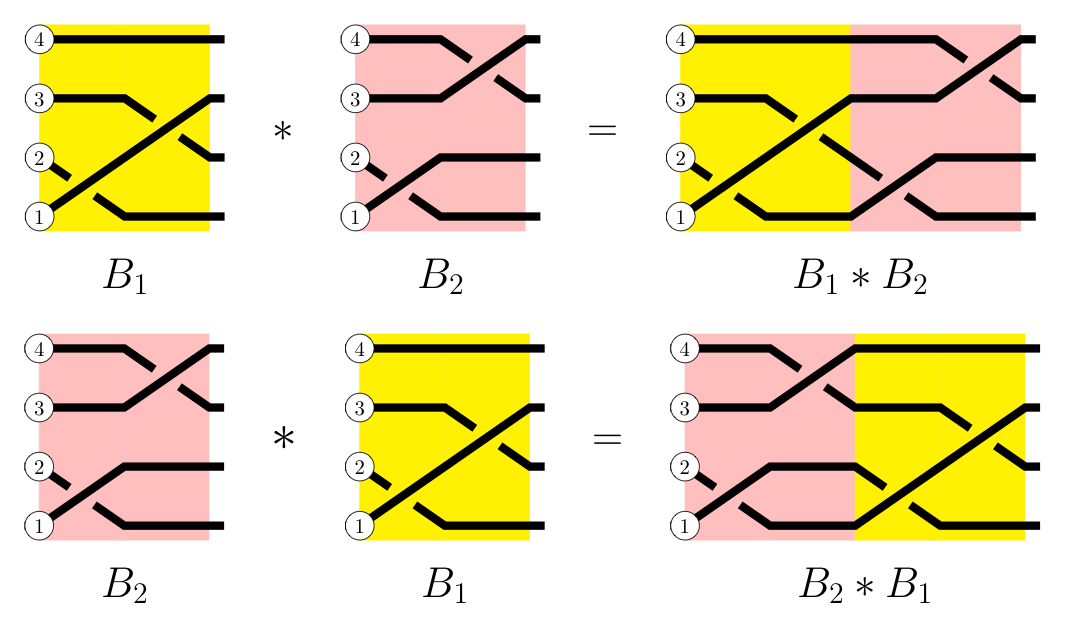
\includegraphics[width=0.6\textwidth]{figures/chapters/1_def_grupo/no_conmutativa.png}
    \caption{Demostración de no conmutatividad en trenzas. Fuente: \cite{ArithmeticBraids}}
    \label{fig:elemento_inverso_proceso}
\end{figure}

% Ejemplo Visual de No Conmutatividad:
% \begin{itemize}
%     \item Consideremos dos cruces básicos: \(\sigma_1\) y \(\sigma_2\). Si aplicamos primero \(\sigma_1\) y luego \(\sigma_2\), obtenemos una trenza diferente a si aplicamos primero \(\sigma_2\) y luego \(\sigma_1\).
%     \item En el primer caso, el hilo \(1\) cruza sobre \(2\) antes de que \(2\) cruce sobre \(3\). En el segundo caso, el orden es inverso, lo cual produce una estructura de trenza distinta. Esto se puede ver claramente en los diagramas adjuntos.
% \end{itemize}

% Esta falta de conmutatividad es fundamental para la estructura del grupo de trenzas y distingue a \( B_n \) de otros grupos, como el grupo simétrico \( S_n \), en el que el orden de las permutaciones no afecta el resultado final.
